\documentclass[12pt,landscape]{article}

%Incantation for swapping landscape/seascape
\special{! TeXDict begin /landplus90{true}store end }

\usepackage[utf8]{inputenc}
\usepackage{amssymb}
\usepackage{stmaryrd}
\usepackage{textcomp}
\usepackage[cm]{fullpage}
\usepackage{t1enc}
\usepackage{amsmath}
\usepackage{url}
\usepackage{graphics}
\usepackage[all]{xy}
\usepackage{tikz, tikz-cd}
% Use the patterns library to draw the cubes figure
\usetikzlibrary{patterns}
\xyoption{2cell}
\UseAllTwocells

\newcommand\whitecol[1]{\textcolor{white}{#1}}


% Color palette
\usepackage{xcolor}
\usepackage{yfonts}

\definecolor{white}{HTML}{FFFFFF}
\definecolor{gray80}{rgb}{0.2, 0.2, 0.2}
\definecolor{gray65}{rgb}{0.35, 0.35, 0.35}
\definecolor{gray30}{rgb}{0.70, 0.70, 0.70}
\definecolor{raspeberry}{HTML}{BF3343}
\definecolor{strawberry}{HTML}{D86E7A}
\definecolor{hlcolor}{HTML}{FBEFF1}
\definecolor{yaleblue}{HTML}{054A91}

% Color palette 2
\definecolor{russian-green}{HTML}{69995D}
\definecolor{chestnut}{HTML}{98473E}
\definecolor{indian-yellow}{HTML}{DB9D47}
\definecolor{carolina}{HTML}{009FFD}
\definecolor{spanish-blue}{HTML}{296EB4}

\makeatletter
\newcommand{\Overrightarrow}[2]{\raisebox{#1}{$\ext@arrow 0359\Rightarrowfill@{\mbox{${#2}$}}{}$}}
\newcommand{\Overleftarrow}[2]{\raisebox{#1}{$\ext@arrow 0359\Leftarrowfill@{\mbox{${#2}$}}{}$}}
%\newcommand{\Overrightarrow}[1]{\raisebox{1.4ex}{$\ext@arrow 0359\Rightarrowfill@{\mbox{${#1}$}}{}$}}
\makeatother

\newenvironment{myitemize}
{\begin{list}{}{
  % Horizontal spaces
%  \setlength{\rightmargin}{0pt} % ?
%  \setlength{\listparindent}{0pt} % ?
  \setlength{\labelwidth}{5pt} % Global indentation reserved for label
  \setlength{\labelsep}{5pt} % How far is the label on the left of paragraph
  \setlength{\leftmargin}{10pt} % should be labelwidth + labelsep
  \setlength{\parindent}{0pt} % Indentation of next paragraphs of the item
  \setlength{\itemindent}{0pt} % Indentation of the first line of item
  % Vertical spaces
  \setlength{\parskip}{8pt} % Distance between two paragraphs or item
  \setlength{\itemsep}{2pt} % Extra distance between two items
  \setlength{\parsep}{10pt}}}
{\end{list}}

\newcommand{\highlight}[1]{{\em #1}}

\newcommand{\Type}{\mathsf{Type}}
\newcommand{\Set}{\mathsf{Set}}
\newcommand{\Prop}{\mathsf{Prop}}
\newcommand{\refl}[1]{\mathsf{refl}\,{#1}}
\newcommand{\mkmlidtype}[3]{{#1} =^{\mathrm{id}}_{#2} {#3}}
\newcommand{\mkmleqdep}[3]{{#1} =^{\mathrm{dep}}_{#2} {#3}}
\newcommand{\hrefl}[1]{\mathsf{refl^{\mathrm{dep}}}\,{#1}}
\newcommand{\mluniv}{\mathsf{U}}
\newcommand{\Jdep}[2]{\mathsf{J}\;{#1}\;{#2}}

\newcommand{\nth}[1]{{#1}^{\mbox{\scriptsize th}}}
\newcommand{\binomial}[2]{\left(\begin{array}{c}#1\\#2\end{array}\right)}

\newcommand{\wfctx}[1]{{#1}~\mathsf{ok}}

\newcommand{\mkover}[1]{\widetilde{#1}}
\newcommand{\mkoverdim}[2]{\widetilde{#2}^{#1}}
%\newcommand{\mkover}[1]{\dot{#1}}
\newcommand{\mkprod}[3]{\Pi {#1}\!:\!{#2}.\,{#3}}
\newcommand{\mkprodovereq}[3]{\mkover{\Pi} {#1}\!:\!{#2}.\,{#3}}
\newcommand{\mkprodovereqopp}[3]{\opp{\mkover{\Pi}} {#1}\!:\!{#2}.\,{#3}}
\newcommand{\mkboundedprod}[4]{\Pi {#3}\!:\!{#1}\leq{#2}.\,{#4}}
\newcommand{\mklam}[3]{\lambda {#1}\!:\!{#2}.\,{#3}}
\newcommand{\mkboundedlam}[4]{\lambda {#3}\!:\!{#1}\leq{#2}.\,{#4}}
\newcommand{\mkapp}[2]{{#1}\,{#2}}
\newcommand{\prodsort}[2]{\Pi ({#1},{#2})}

% selecting kind of treatment of sorts
\newcommand{\typeorsort}[2]{{#2}}

\newcommand{\mksigma}[3]{\Sigma {#1}\!:\!{#2}.\,{#3}}
\newcommand{\mksigmaovereq}[3]{\mkover{\Sigma} {#1}\!:\!{#2}.\,{#3}}
\newcommand{\mksigmaovereqopp}[3]{\opp{\mkover{\Sigma}} {#1}\!:\!{#2}.\,{#3}}
\newcommand{\mkpair}[2]{\langle{#1},{#2}\rangle}
\newcommand{\mkfst}[1]{{#1}.1}
\newcommand{\mksnd}[1]{{#1}.2}
\newcommand{\sigsort}[2]{\Sigma ({#1},{#2})}

\newcommand{\sortsort}[1]{{\mathcal S}_{#1}}

\newcommand{\Sone}{\mathbb{S}^1}
\newcommand{\casesone}[5]
  {\mathsf{case}\;{#1}\;\mathsf{of}\;{#2}\;\Rightarrow\;{#3}\;|\;{#4}\;\Rightarrow\;{#5}\;\mathsf{end}}
\newcommand{\base}{\mathsf{base}}
\newcommand{\loopsone}{\mathsf{loop}}
\newcommand{\Sonesort}{l_{\mathbb{S}^1}}

\newcommand{\emptyctx}{\emptyset}

\newcommand{\sort}[1]{\mathsf{Type}_{#1}}
\newcommand{\istype}{~:~\mluniv}

\newcommand{\mkeq}[3]{{#1} =_{#2} {#3}}
\newcommand{\mkhomeq}[3]{{#1} =_{#2} {#3}}
\newcommand{\mkeqovereq}[3]{{#1} \,\mkover{=}_{#2}\, {#3}}
\newcommand{\mkeqovereqdim}[4]{{#2} \,\mkoverdim{#1}{=}_{#3}\, {#4}}
\newcommand{\mkeqtype}[3]{{#1} =_{#2} {#3}} % case where we can write either s or refl{s}
\newcommand{\mkeqtypeovereq}[3]{{#1} \,\mkover{=}_{#2}\, {#3}} % case where we can write either s or refl{s}
\newcommand{\mkeqarray}[3]{\begin{array}{c}{#1}\\ =_{#2}\\ {#3}\end{array}}
\newcommand{\mkfaces}[3]{\mkeq{#1}{#2}{#3}}
\newcommand{\mkfacesarray}[3]{\mkeqarray{#1}{#2}{#3}}
\newcommand{\mkfacesover}[3]{\mkeqovereq{#1}{#2}{#3}}
\newcommand{\lameq}[2]{\lambda {#1}.{#2}}
%\newcommand{\reflterm}[1]{\textsf{refl}{#1}}
\newcommand{\reflterm}[1]{\widehat{#1}}
\newcommand{\overreflterm}[1]{{\mkover{\reflterm{#1}}}}
\newcommand{\minirefltermdim}[2]{{{\widehat{#2}}^{\raisebox{1mm}{\normalsize #1}}}}
\newcommand{\refltermdim}[2]{\widehat{#2}^{#1}}
%\newcommand{\reflterm}[1]{\lambda{#1}}
%\newcommand{\refltype}[1]{\lambda{#1}}
\newcommand{\refltype}[1]{\reflterm{#1}}
\newcommand{\purerewlr}[1]{\overrightarrow{#1}}
\newcommand{\purerewrl}[1]{\overleftarrow{#1}}
%\newcommand{\rewlr}[2]{\mathsf{rew}^\rightarrow\;{#1}\;\mathsf{in}\;{#2}}
%\newcommand{\rewrl}[2]{\mathsf{rew}^\leftarrow\;{#1}\;\mathsf{in}\;{#2}}
\newcommand{\rewlrmap}[1]{\overrightarrow{#1}}
\newcommand{\rewrlmap}[1]{\overleftarrow{#1}}
\newcommand{\rewlr}[2]{\overrightarrow{#1}(#2)}
\newcommand{\rewrl}[2]{\overleftarrow{#1}(#2)}
\newcommand{\deprewlr}[1]{\raisebox{0em}{$\ulcorner$}\!#1}
\newcommand{\minideprewlr}[1]{\raisebox{0em}{$\ulcorner$}\!\!\!#1}
\newcommand{\deprewrl}[1]{{#1}\raisebox{-0.2em}{$\!\lrcorner$}}
\newcommand{\rewlrspec}[2]{{#1}^{\rightarrow}(#2)}
\newcommand{\rewrlspec}[2]{{#1}^{\leftarrow}(#2)}
\newcommand{\rewlrrevspec}[2]{{#1}_-^{\rightarrow}(#2)}
\newcommand{\rewrlrevspec}[2]{{#1}_-^{\leftarrow}(#2)}
\newcommand{\rewlrrevspecin}[2]{{#1}_+^{\rightarrow}(#2)}
\newcommand{\rewrlrevspecin}[2]{{#1}_+^{\leftarrow}(#2)}
\newcommand{\doublerewlr}[2]{\Overrightarrow{1.4ex}{#1}({#2})}
\newcommand{\doublerewrl}[2]{\Overleftarrow{1.4ex}{#1}({#2})}
\newcommand{\doublerewlrmap}[1]{\Overrightarrow{1.4ex}{#1}}
\newcommand{\doublerewrlmap}[1]{\Overleftarrow{1.4ex}{#1}}
\newcommand{\cohrewlr}[2]{\mathsf{coh}{#1}({#2})}
%\newcommand{\mktuple}[6]{\{#1\mapsto #3(#1); #2\mapsto #4(#2); #1\mapsto #5(#1); #2\mapsto #6(#2)\}}
\newcommand{\mktuple}[6]{\{#3; #4; #5; #6\}_{#1,#2}}
\newcommand{\mkcohtuple}[7]{\{#3; #4; #5; #6; #7\}_{#1,#2}}
\newcommand{\mktupleshort}[6]{\{#3; #4; #5; #6\}}
\newcommand{\mktupleshortnamed}[6]{\{#3; #4; #5; #6\}_{#1,#2}}
\newcommand{\opp}[1]{{#1}^{-1}}
\newcommand{\oppi}[2]{\appi{#1}{(\opp{#2}/{#2})}}

\newcommand{\weakensquarelr}[1]{{#1}_L}
\newcommand{\weakensquarerl}[1]{{#1}_R}
\newcommand{\weakensquarelrmap}[1]{{#1}_L}
\newcommand{\weakensquarerlmap}[1]{{#1}_R}

\newcommand{\rewlrmkeq}[4]{\mkeq{\rewlr{#1}{#2}}{#3}{#4}}

% Version basse
%% \newcommand{\appi}[2]{{#1}_{#2}}
%% \newcommand{\appidep}[2]{{#1}_{({#2})}}
%% \newcommand{\bp}[1]{{#1}_0}
%% \newcommand{\ep}[1]{{#1}_1}
%% \newcommand{\bpdep}[1]{{#1}_{(0)}}
%% \newcommand{\epdep}[1]{{#1}_{(1}}}
% Version haute
% \newcommand{\metaappi}[2]{{#1}_{[{#2}]}}
\newcommand{\appi}[2]{{#1}\;\!{#2}}
\newcommand{\appidep}[2]{{#1}_{#2}}
\newcommand{\bp}[1]{{#1}{\scriptstyle 0}}
\newcommand{\ep}[1]{{#1}{\scriptstyle 1}}
\newcommand{\bpoverdim}[2]{{#2}{\scriptstyle \mkoverdim{#1}{0}}}
\newcommand{\epoverdim}[2]{{#2}{\scriptstyle \mkoverdim{#1}{1}}}
\newcommand{\bpdep}[1]{{#1}_0}
\newcommand{\epdep}[1]{{#1}_1}

\newcommand{\bpsubstexpl}[2]{{#2}_{\{0/{#1}\}}}
\newcommand{\epsubstexpl}[2]{{#2}_{\{1/{#1}\}}}
\newcommand{\eqsubstexpl}[2]{{#2}_{\{\star/{#1}\}}}
\newcommand{\bpsubstexplcons}[2]{{#2}\}\{0/{#1}}
\newcommand{\epsubstexplcons}[2]{{#2}\}\{1/{#1}}
\newcommand{\eqsubstexplcons}[2]{{#2}\}\{\star/{#1}}
\newcommand{\bpsubst}[2]{{#2}{[0/{#1}]}}
\newcommand{\epsubst}[2]{{#2}{[1/{#1}]}}
\newcommand{\bpsubstctx}[3]{{#3}{[0/{#2}]}^{#1}}
\newcommand{\epsubstctx}[3]{{#3}{[1/{#2}]}^{#1}}
\newcommand{\takebpface}[2]{\partial^{#1}_0{#2}}
\newcommand{\takeepface}[2]{\partial^{#1}_1{#2}}

\newcommand{\dimvalid}[2]{{#1} \in {#2}}
\newcommand{\dimdeclare}[1]{{#1}}
\newcommand{\dimlength}[1]{|#1|_{\mathit{dim}}}
\newcommand{\dimindex}[2]{\#_{#1}{#2}}

\newcommand{\substminus}[2]{{#1}-{#2}}
\newcommand{\substminusbernardymoulin}[2]{{#1}/{#2}}

\newcommand{\N}{\mathbb{N}}
\newcommand{\expand}[2]{\mathsf{expand}(#1,#2)}

\newcommand{\defeq}{\triangleq}
%\newcommand{\metaequiv}{=\!\!\!=}
\newcommand{\metaequiv}{\cong}
\newcommand{\metaletin}[3]{\mathit{let}\;{#1}\;\defeq\;{#2}\;\mathit{in}\;{#3}}
\newcommand{\map}[2]{\mathsf{ap}\,{#1}\,{#2}}
\newcommand{\depmap}[2]{\mathsf{apd}\,{#1}\,{#2}}
\newcommand{\transport}[3]{\mathsf{transport}\,{#1}\,{#2}\,{#3}}
\newcommand{\deptransport}[3]{\mathsf{transportd}\,{#1}\,{#2}\,{#3}}
%\newcommand{\swap}[1]{\mathsf{swap}(#1)}
%\newcommand{\swapbracket}[1]{\mathsf{swap}(#1)}
%\newcommand{\swaptype}[1]{\mathsf{swap}(#1)}
\newcommand{\swap}[1]{{#1}^{\circ}}
\newcommand{\swapbracket}[1]{({#1})^{\circ}}
\newcommand{\swaptype}[1]{{#1}^{\circ}}
\newcommand{\swapoverdim}[2]{{#2}^{\mkoverdim{#1}{\circ}}}
\newcommand{\homsquare}[1]{\mathsf{homsquare}(#1)}
\newcommand{\permute}[2]{\mathsf{permute}_{#1}(#2)}
\newcommand{\adjacenttranspose}[2]{\sigma_{#1}({#2})}
\newcommand{\swapprodeq}[2]{\mathsf{swap}_{\Pi=}^{#1}(#2)}
\newcommand{\swapeqprod}[2]{\mathsf{swap}_{=\Pi}^{#1}(#2)}
\newcommand{\swapeqprodlr}[2]{\mathsf{swap}_{=\Pi}^{\rightarrow}({#1})(#2)}
\newcommand{\swapeqprodrl}[2]{\mathsf{swap}_{=\Pi}^{\leftarrow}({#1})(#2)}
\newcommand{\swapsigmaeq}[1]{\mathsf{swap}_{\Sigma=}(#1)}
\newcommand{\swapeqsigma}[1]{\mathsf{swap}_{=\Sigma}(#1)}

\newcommand{\bool}{\mathsf{bool}}
\newcommand{\booldeux}{\bool^2}
\newcommand{\boolexp}{\bool^{\bool}}

\newcommand{\reduce}{\;\triangleright\;}

\newcommand{\emptysubst}{\emptyctx}

\newcommand{\sortrule}{\sort{}}
\newcommand{\axrule}{\mathsf{Ax}}
\newcommand{\ctxemptyrule}{\mathsf{Ctx}_{\emptyctx}}
\newcommand{\ctxconsrule}{\mathsf{Ctx}_{\mathsf{cons}}}
\newcommand{\convrule}{\mathsf{Conv}}
\newcommand{\convruleredright}{\reduce_R}
\newcommand{\convruleredleft}{\reduce_L}
\newcommand{\convrulerefl}{\equiv_{\mathsf{refl}}}
\newcommand{\convruletrans}{\equiv_{\mathsf{trans}}}

\newcommand{\circovereq}{\;\mkover{\circ}\;}
\newcommand{\circsigma}{\circ_{\Sigma}}

\newcommand{\comprule}{R_{\mathsf{\circ}}}
\newcommand{\opprule}{R_{\mathsf{\opp}}}

\newcommand{\idleftredrule}{\mathsf{Id_L}}
\newcommand{\idrightredrule}{\mathsf{Id_R}}
\newcommand{\idoppredrule}{\mathsf{\opp{Id}}}
\newcommand{\oppoppredrule}{\mathsf{\opp{(\opp{\_})}}}
\newcommand{\assoccompredrule}{\mathsf{Assoc}}
\newcommand{\distriboppcompredrule}{\mathsf{\opp{\circ}}}
\newcommand{\squaredownredrule}{\circ_{=_{\mkover{=}}}}
\newcommand{\exchangerule}{\mathsf{Exch}}
\newcommand{\compeqovereqredrule}{\circ_{\mkover{=}}}
\newcommand{\squareprodredrule}{\circ_{=_{\mkover{\Pi}}}}

\newcommand{\depmapdef}{\mathsf{ApD}}
\newcommand{\funextpuredef}{\mathsf{LiftDim}}
\newcommand{\funextdeppuredef}{\mathsf{LiftDepDim}}
\newcommand{\funextdepdeppuredef}{\mathsf{LiftDepDim}}
\newcommand{\funextdef}{\mathsf{FunExt}}
\newcommand{\funextdepdef}{\mathsf{FunDepExt}}
\newcommand{\funext}[1]{\mathsf{funext}(#1)}
\newcommand{\funextdep}[1]{\mathsf{fundepext}(#1)}
\newcommand{\funextpure}[1]{\mathsf{liftdim}(#1)}
\newcommand{\funextdeppure}[1]{\mathsf{liftdepdim}(#1)}

\newcommand{\partialcubset}[2]{\mathsf{\nu set}_{#1}^{<#2}}
\newcommand{\mycubset}[1]{\mathsf{\nu Set}_{#1}}
\newcommand{\mycubsetfrom}[2]{\mathsf{\nu set}_{#1}^{\geq#2}}
\newcommand{\mycubsetcomp}[2]{\mathsf{\nu set}_{#1}^{=#2}}
\newcommand{\mybox}[1]{\mathsf{frame}_{#1}}
\newcommand{\mylayer}[1]{\mathsf{layer}_{#1}}
\newcommand{\mycube}[1]{\mathsf{painting}_{#1}}
\newcommand{\myfullbox}[1]{\mathsf{fullframe}_{#1}}
\newcommand{\unitpoint}{\star}
\newcommand{\unittype}{\mathsf{unit}}
\newcommand{\hd}{\mathsf{hd}}
\newcommand{\tl}{\mathsf{tl}}
\newcommand{\downbox}[2]{\mathsf{restrframe}_{#1,#2}}
\newcommand{\downlayer}[2]{\mathsf{restrlayer}_{#1,#2}}
\newcommand{\downcube}[2]{\mathsf{restrpainting}_{#1,#2}}
\newcommand{\cohbox}[2]{\mathsf{cohframe}_{#1,#2}}
\newcommand{\cohlayer}[2]{\mathsf{cohlayer}_{#1,#2}}
\newcommand{\cohcube}[2]{\mathsf{cohpainting}_{#1,#2}}


\newcommand{\mkeqsquare}[5]{\begin{array}{c}{#1} ~~=~~ {#5}\\[-0.2cm] ~~\mbox{}_{\mkeqovereq{#2}{#3}{#4}}\\\end{array}}
\newcommand{\mkeqcube}[7]{\begin{array}{c}{#1} ~~=~~ {#7}\\[-0.2cm] ~~\mbox{}_{#2~\mkover{=}~#6}\\[-0.2cm] ~~~~~\;\mbox{}_{\mbox{}_{\mkeqovereqdim{2}{#3}{#4}{#5}}}\\\end{array}}
\newcommand{\xysquare}[9]{
  \xymatrix{
  {#1} \ar_{#5}[dd] \ar^{#7}[rrr] & & & \ar^{#6}[dd] {#3}\\
  *\txt<4pc>{} \ar^{#9}@{=>}[rrr] & & & *\txt<4pc>{}\\
  {#2} \ar^{#8}[rrr] & & & {#4}}
}

\begin{document}
\begin{LARGE}
\begin{sf}

\mbox{}
\vspace{3cm}

\begin{center}

\textcolor{red}{\Huge About the construction of simplicial and cubical
  sets in indexed form:\\ the case of degeneracies}

\medskip
\bigskip
\bigskip
{\Large Hugo Herbelin and Ramkumar Ramachandra}

\bigskip
\bigskip
\bigskip
\bigskip
\bigskip
\bigskip
\bigskip
TYPES 2025

\bigskip
\bigskip
Glasgow
\bigskip

10 June 2025

\bigskip
\bigskip

\end{center}

\newcommand{\mysem}[1]{\llbracket #1 \rrbracket}
\newcommand{\deppsh}[2]{\mathsf{DepPresheaf}(#1,#2)}
\newcommand{\HSet}[1]{\mathsf{HSet}}
\newcommand{\imp}{\rightarrow}

%%%%%%%%%%%%%%%%%%%%%%%%%%%%%%%%%%%%%%%%%%%%%%%%%%%%%%%%%%%%%%%%%%%%%%
\newpage

\begin{center}
\textcolor{red}{\huge The problem of \emph{semi-simplicial types}}
\end{center}

\bigskip
\bigskip
Construct the following family of family types in homotopy type theory:

$$
\begin{array}{cllccllll}
X_0 & : & \Type & \mbox{(points)}\\
\\
X_1 & : & X_0 \times X_0 \rightarrow \Type & \mbox{(segments)}\\
\\
X_2 & : & \Pi x_1x_2x_3.\, X_1 (x_1,x_2) \imp X_1 (x_1,x_3) \imp X_1 (x_2,x_3)\rightarrow \Type \qquad & \mbox{(triangles)}\\
\\
\vdots\\
\end{array}
$$

%%%%%%%%%%%%%%%%%%%%%%%%%%%%%%%%%%%%%%%%%%%%%%%%%%%%%%%%%%%%%%%%%%%%%%
\newpage

\begin{center}
\textcolor{red}{\huge The problem of \emph{semi-simplicial types}}
\end{center}

\bigskip
\bigskip
Construct the following family of family types in pure type theory:

$$
\begin{array}{cllccllll}
X_0 & : & \Type & \mbox{(points)}\\
\\
X_1 & : & X_0 \times X_0 \rightarrow \Type & \mbox{(segments)}\\
\\
X_2 & : & \Pi x_1x_2x_3.\, X_1 (x_1,x_2) \imp X_1 (x_1,x_3) \imp X_1 (x_2,x_3)\rightarrow \Type \qquad & \mbox{(triangles)}\\
%X_2 & : & \Pi (x_{LL},x_{LR}).\, X_1 (x_{LL},x_{LR}) \imp\\
%& & \Pi (x_{RL},x_{RR}).\, X_1 (x_{RL},x_{RR}) \imp\\
%& & X_1 (x_{LL},x_{RL}) \times X_1 (x_{LR},x_{RR}) \rightarrow \Type \qquad & \mbox{(squares)}\\
\\
\vdots\\
\end{array}
$$
\bigskip

$\!\!\!\!\!\!\!\!\!\!\!\!\!\!\!$\begin{tikzcd}
      & \mbox{$\!\!\!\!\!\!\!\!\!\!\!\!$two problems into one$\!\!\!\!\!\!\!\!\!\!\!\!$} \arrow[ld] \arrow[rd]\\
\begin{tabular}{c}\mbox{semi-simplicial \emph{types}}\\$\left(\begin{tabular}{c}needs -- at least -- a \\description of higher-\\dimensional coherences\end{tabular}\right)$\end{tabular}\!\!\!\!\!\!\!\!& & \begin{tabular}{c}recipe for \emph{indexed} semi-simplicial\\
$\left(\begin{tabular}{c}this talk, for $\HSet{}$,\\see also Voevodsky, Part-Luo,\\
 Altenkirch-Capriotti-Kraus \end{tabular}\right)$
\end{tabular}\qquad\qquad\\
\end{tikzcd}

%%%%%%%%%%%%%%%%%%%%%%%%%%%%%%%%%%%%%%%%%%%%%%%%%%%%%%%%%%%%%%%%%%%%%%
\newpage

\begin{center}
\textcolor{red}{\huge The fibred/indexed correspondence for $\HSet{}$}
\end{center}

\bigskip
\bigskip
\bigskip
\bigskip
\bigskip
For $B:\HSet{l}$

$$\begin{array}{c}E:\HSet{l}\\[5mm]\bigg\downarrow\\[1cm] B
\end{array}
~~~\simeq~~~ B \rightarrow \HSet{l}$$

%%%%%%%%%%%%%%%%%%%%%%%%%%%%%%%%%%%%%%%%%%%%%%%%%%%%%%%%%%%%%%%%%%%%%%
\newpage

\begin{center}
\textcolor{red}{\huge Iterating the fibred/indexed correspondence for $\HSet{}$}
\end{center}

\bigskip
\bigskip

\noindent Application to definition of Reedy presheaves in \emph{indexed form}, here for semi-cubical sets:

$$
\begin{array}{cllccllll}
\multicolumn{3}{c}{\mbox{\emph{fibred form}}} & \qquad\mathit{vs}\qquad & \multicolumn{3}{l}{\mbox{\emph{indexed form}}} \\
Y_0 &:& \HSet{l} & & X_0 & : & \HSet{l} & \mbox{(points)}\\[5mm]
\bigg\uparrow {\mbox{\Large $d^L$}}\bigg\uparrow{\mbox{\Large $d^R$}}\\[8mm]
Y_1 &:& \HSet{l} & & X_1 & : & X_0 \times X_0 \rightarrow \HSet{l} & \mbox{(segments)}\\[5mm]
\bigg\uparrow{\mbox{\Large $d^{L\star}$}}\bigg\uparrow{\mbox{\Large $d^{R\star}$}}\bigg\uparrow{\mbox{\Large $d^{\star L}$}}\bigg\uparrow{\mbox{\Large $d^{\star R}$}} \\[8mm]
Y_2 &:& \HSet{l} & & X_2 & : & \Pi (x_{LL},x_{LR}).\, \Pi x_{L*}:X_1 (x_{LL},x_{LR}).\\
& & & & & & \Pi (x_{RL},x_{RR}).\, \Pi x_{R*}:X_1 (x_{RL},x_{RR}).\, \\
\multicolumn{3}{c}{\mbox{~+ coherences}} & & & & X_1 (x_{LL},x_{RL}) \times X_1 (x_{LR},x_{RR}) \rightarrow \HSet{l} \qquad & \mbox{(squares)}\\
%\\
%\vdots & & & & \vdots\\
\end{array}
$$

%%%%%%%%%%%%%%%%%%%%%%%%%%%%%%%%%%%%%%%%%%%%%%%%%%%%%%%%%%%%%%%%%%%%%%
\newpage

\begin{center}
\textcolor{red}{\huge Iterating the fibred/indexed correspondence for $\HSet{}$}
\end{center}

\bigskip
\bigskip

\noindent Application to the definition of Reedy presheaves in \emph{indexed form}, here for cubical sets:

$$
\begin{array}{cllccllll}
\multicolumn{3}{c}{\mbox{\emph{fibred form}}} & \qquad\mathit{vs}\qquad & \multicolumn{3}{l}{\mbox{\emph{indexed form}}} \\
Y_0 &:& \HSet{l} & & X_0 & : & \HSet{l} & \mbox{(points)}\\[5mm]
\bigg\uparrow {\mbox{\Large $d^L$}}\bigg\uparrow{\mbox{\Large $d^R$}}\\[8mm]
Y_1 &:& \HSet{l} & & X_1 & : & X_0 \times X_0 \rightarrow \HSet{l} & \mbox{(segments)}\\[5mm]
\bigg\uparrow{\mbox{\Large $d^{L\star}$}}\bigg\uparrow{\mbox{\Large $d^{R\star}$}}\bigg\uparrow{\mbox{\Large $d^{\star L}$}}\bigg\uparrow{\mbox{\Large $d^{\star R}$}} \\[8mm]
Y_2 &:& \HSet{l} & & X_2 & : & \Pi (x_{LL},x_{LR}).\, \Pi x_{L*}:X_1 (x_{LL},x_{LR}).\\
& & & & & & \Pi (x_{RL},x_{RR}).\, \Pi x_{R*}:X_1 (x_{RL},x_{RR}).\, \\
\multicolumn{3}{c}{\mbox{~+ coherences}} & & & & X_1 (x_{LL},x_{RL}) \times X_1 (x_{LR},x_{RR}) \rightarrow \HSet{l} \qquad & \mbox{(squares)}\\
%\\
%\vdots & & & & \vdots\\
\end{array}
$$

Motivations:

1. The iterated fibred/indexed correspondence is interesting in itself

2. Suggests models of type theory closer to the syntax: e.g. equality
interpreted as a (relevant) relation rather than as a span

%%%%%%%%%%%%%%%%%%%%%%%%%%%%%%%%%%%%%%%%%%%%%%%%%%%%%%%%%%%%%%%%%%%%%%
\newpage

\begin{center}
\textcolor{red}{\huge Rest of the talk}
\end{center}

\bigskip
\noindent Presheaves in ``indexed'' form
\bigskip

\noindent - following a $n$-ary ``parametricity'' recipe
\bigskip

 - s.t. \emph{unary} parametricity gives augmented semi-simplicial sets
\bigskip

 - and \emph{binary} parametricity gives semi-cubical sets
\bigskip

\noindent - equipped with a \emph{degeneracy}
\bigskip

\noindent - machine-checked in Rocq

%% \mbox{}

%% \vspace{5cm}

%% \begin{center}
%% \textcolor{red}{\huge Investigations into syntactic iterated parametricity and cubical type theory
%% Towards syntactic ``indexed'' models of various cubical/parametric type theories}
%% \end{center}

\iffalse
%%%%%%%%%%%%%%%%%%%%%%%%%%%%%%%%%%%%%%%%%%%%%%%%%%%%%%%%%%%%%%%%%%%%%%
\newpage

\begin{center}
\textcolor{red}{\huge Presheaf models of homotopy type theory in indexed form: motivation}
\end{center}

\bigskip

Different approaches, different traditions:
\bigskip

\begin{tabular}{ccc}
``Semantic'' (presheaf) models & vs & ``Syntactic'' models\\
\\
$
\begin{array}{l}
\vdash_{ZF} ((\Gamma \vdash_{TT} A) \rightarrow \deppsh{\Gamma}{A})\\
\vdash_{TT} ((\Gamma \vdash_{TT} A) \rightarrow \deppsh{\Gamma}{A})\\
\end{array}
$ & &
$\vdash_{PRA} ((\Gamma \vdash_{TT} A) \rightarrow (\vdash_{ETT} \deppsh{\Gamma}{A})$\\
\\
& & separation of concerns \\
close to the ``mental'' intuitions & &
protects from a ``set-theoretic'' bias\\
& & metalanguage does not leak\\
\end{tabular}

\bigskip
Reedy presheaves in (usual) ``fibred'' form vs Reedy presheaves in ``indexed'' form

Advantages:
Relatively simple definition
Well-studied

Advantages:
Closer to the syntax, liable to better preserve definitional equalities
Interesting in itself
\fi

\newcommand{\Obj}{\ensuremath{\mathsf{Obj}}}
\newcommand{\Hom}{\ensuremath{\mathsf{Hom}}}
\newcommand{\id}{\ensuremath{\mathsf{id}}}

%%%%%%%%%%%%%%%%%%%%%%%%%%%%%%%%%%%%%%%%%%%%%%%%%%%%%%%%%%%%%%%%%%%%%%
\newpage

\begin{center}
\textcolor{red}{\huge A uniform approach to augmented simplicial sets and cubical sets}
\end{center}

%It seems today ``folklore'' that the augmented simplicial and cubical
%categories only differ in the ``arity'' of a finite set $\nu$:

\medskip

Augmented simplicial and cubical categories only differ in the
``arity'' of a finite set $\nu$:

$$
  \begin{array}{ll}
    \Obj       & := \mathbb{N}\\
    \Hom(p, n) & := \{l \in (\nu \sqcup \{\star\})^n \mid \text{number of $\star$ in $l = p$}\} \\
    g \circ f             & :=
    \begin{cases}
      f                & \text{if $g = \epsilon$}                                                   \\
      a\,(g' \circ f)  & \text{if $g = a\,g'$}, \text{where $a \in \nu$}                            \\
      a\,(g' \circ f') & \text{if $g = \star\,g'$, $f = a\,f'$, where $a \in \nu$ or $a = \star$} \\
    \end{cases}            \\
    \id                   & := \star \ldots \star \text{ $n$ times for $\id \in \Hom(n, n)$}
  \end{array}
$$

\medskip
\begin{center}
\begin{tabular}{ccc}
\textcolor{white}{augmented semi-simplicial sets with $\nu = \{0\}$} & &
\textcolor{white}{semi-cubical sets with $\nu = \{L,R\}$}\\
\textcolor{white}{(counting from -1)} & &\textcolor{white}{(counting from 0)}\\[-5mm]
\\
\\
\\
\\
\\
\\
\\
\\
\end{tabular}
\end{center}

%%%%%%%%%%%%%%%%%%%%%%%%%%%%%%%%%%%%%%%%%%%%%%%%%%%%%%%%%%%%%%%%%%%%%%
\newpage

\begin{center}
\textcolor{red}{\huge A uniform approach to augmented simplicial sets and cubical sets}
\end{center}

%It seems today ``folklore'' that the augmented simplicial and cubical
%categories only differ in the ``arity'' of a finite set $\nu$:

\medskip

Augmented simplicial and cubical categories only differ in the
``arity'' of a finite set $\nu$:

$$
  \begin{array}{ll}
    \Obj       & := \mathbb{N}\\
    \Hom(p, n) & := \{l \in (\nu \sqcup \{\star\})^n \mid \text{number of $\star$ in $l = p$}\} \\
    g \circ f             & :=
    \begin{cases}
      f                & \text{if $g = \epsilon$}                                                   \\
      a\,(g' \circ f)  & \text{if $g = a\,g'$}, \text{where $a \in \nu$}                            \\
      a\,(g' \circ f') & \text{if $g = \star\,g'$, $f = a\,f'$, where $a \in \nu$ or $a = \star$} \\
    \end{cases}            \\
    \id                   & := \star \ldots \star \text{ $n$ times for $\id \in \Hom(n, n)$}
  \end{array}
$$

\medskip
\begin{center}
\begin{tabular}{ccc}
augmented semi-simplicial sets with $\nu = \{0\}$ & &
semi-cubical sets with $\nu = \{L,R\}$\\
\textcolor{black}{(counting from -1)} & &\textcolor{black}{(counting from 0)}\\[-5mm]
\\
    \begin{tikzcd}
      & |[alias=F]|00\star \arrow[ddr, dash, "0\star\star"] & \\\\
      \star00 \arrow[rr, dash, "\star\star0"{name=T, below}]\arrow[uur, dash, "\star0\star"] && 0\star0 \\
      \arrow[rightarrow, from=F, to=T, phantom, "\star\star\star" description]
    \end{tikzcd}
&\qquad\qquad&
    ~~~\begin{tikzcd}
      LR \arrow[r, dash, "\star R"{name=F}] \arrow[d, dash, "L\star" left] & RR \arrow[d, dash, "R\star"] \\
      LL \arrow[r, dash, "\star L"{name=T, below}] & RL \\
      \arrow[rightarrow, from=F, to=T, phantom, "\star\star" description]
    \end{tikzcd}\\[0mm]
\end{tabular}
\end{center}


%%%%%%%%%%%%%%%%%%%%%%%%%%%%%%%%%%%%%%%%%%%%%%%%%%%%%%%%%%%%%%%%%%%%%%
\newpage

\begin{center}
\textcolor{red}{\huge An effective indexed construction as a dependent stream of
  dependent sets}
\end{center}

\centerline{$\nu$-sets}

\includegraphics{nusets.png}

\centerline{Truncated $\nu$-sets}

\includegraphics{truncnusets.png}

\bigskip
\bigskip

where $\mathsf{\color{indian-yellow}{fullframe^n_m}}$ is defined by mutual
recursive construction (see next slides)

%%%%%%%%%%%%%%%%%%%%%%%%%%%%%%%%%%%%%%%%%%%%%%%%%%%%%%%%%%%%%%%%%%%%%%
\newpage

\begin{center}
\textcolor{red}{\huge The recursive process used to build frames from layers of paintings}
\end{center}

\bigskip
\bigskip

\begin{center}
  
\begin{tikzpicture}[scale=4]
    \draw[spanish-blue, fill=spanish-blue] (0, 0) -- (1, 0) -- (1, 1) -- (0, 1) -- (0, 0);
    \draw[spanish-blue, fill=spanish-blue, nearly transparent] (0.6, 1) -- (0.6, 1.6) -- (1.6, 1.6) -- (1.6, 0.6) -- (1, 0.6);
  \end{tikzpicture}
  \;\;
  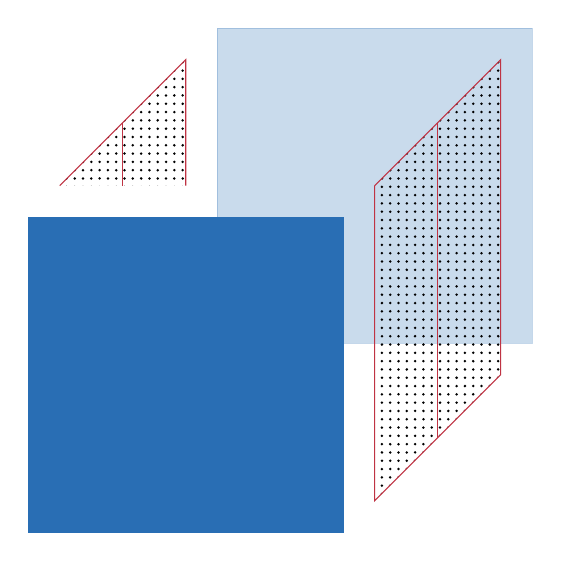
\begin{tikzpicture}[scale=4]
    \draw[spanish-blue, fill=spanish-blue] (0, 0) -- (1, 0) -- (1, 1) -- (0, 1) -- (0, 0);
    \draw[spanish-blue, fill=spanish-blue, nearly transparent] (0.6, 1) -- (0.6, 1.6) -- (1.6, 1.6) -- (1.6, 0.6) -- (1.0, 0.6);
    \draw[raspeberry, pattern=dots] (1.1, 1.1) -- (1.5, 1.5) -- (1.5, 0.5) -- (1.1, 0.1) -- (1.1, 1.1);
    \draw[raspeberry] (1.3, 1.3) -- (1.3, 0.3);
    \draw[raspeberry, pattern=dots] (0.1, 1.1) -- (0.5, 1.5) -- (0.5, 1.1);
    \draw[raspeberry] (0.3, 1.3) -- (0.3, 1.1);
  \end{tikzpicture}
  \;\;
  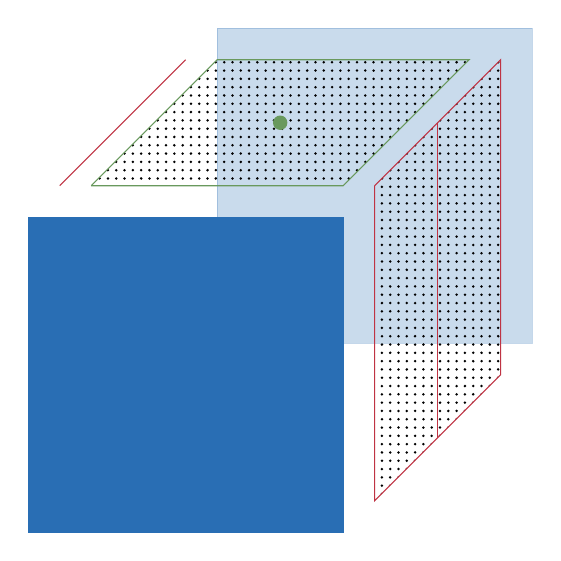
\begin{tikzpicture}[scale=4]
    \draw[spanish-blue, fill=spanish-blue] (0, 0) -- (1, 0) -- (1, 1) -- (0, 1) -- (0, 0);
    \draw[spanish-blue, fill=spanish-blue, nearly transparent] (0.6, 1) -- (0.6, 1.6) -- (1.6, 1.6) -- (1.6, 0.6) -- (1.0, 0.6);
    \draw[raspeberry, pattern=dots] (1.1, 1.1) -- (1.5, 1.5) -- (1.5, 0.5) -- (1.1, 0.1) -- (1.1, 1.1);
    \draw[raspeberry] (1.3, 1.3) -- (1.3, 0.3);
    \draw[raspeberry] (0.1, 1.1) -- (0.5, 1.5);
    \draw[russian-green, pattern=dots] (0.2, 1.1) -- (1.0, 1.1) -- (1.4, 1.5) -- (0.6, 1.5) -- (0.2, 1.1);
    \filldraw[russian-green] (0.8, 1.3) circle (0.6pt);
  \end{tikzpicture}
\end{center}

%%%%%%%%%%%%%%%%%%%%%%%%%%%%%%%%%%%%%%%%%%%%%%%%%%%%%%%%%%%%%%%%%%%%%%
\newpage

\begin{center}
\textcolor{red}{\huge The recursive construction, formally}
\end{center}

\includegraphics{frame.png}

\bigskip

\quad where we need to define
$\mathsf{\color{russian-green}{restr}_{\color{indian-yellow}\mathsf{frame}}}$ (see next slide)

\iffalse
\noindent which corresponds, when $\nu=2$, to
the following organisation of the $3^n$ components of a $n$-cube (shown for $n=2$), with
$\mybox{l}$ associating layers on the left and $\mycube{l}$ associating them
on the right:
$$
\begin{array}{l}
\begin{array}{lll}
\mbox{\textit{squares}}\\
[3mm]\mbox{\textit{lines}}\\
[3mm]\mbox{\textit{points}}\\
[1mm]\end{array}
\framebox{$\begin{array}{lll}
\overbrace{\raisebox{0.05cm}{\framebox{$
\begin{array}{ll}
\raisebox{0cm}{\hspace{.5cm}{\scriptsize$\mylayer{l}^{1,0}$}}  & \framebox{$x_{0\star}$}\\
[1mm]\overbrace{\framebox{$x_{00}$}~\framebox{$x_{01}$}}&
\raisebox{-0.1cm}{{\scriptsize \hspace{0.1cm}$\mycube{l}^{1,0}\!\!\!\!\!\!\!\!$}}
\\
\end{array}
$}}~
{\raisebox{0.05cm}{\framebox{$
\begin{array}{ll}
\raisebox{0cm}{\hspace{.5cm}{\scriptsize$\mylayer{l}^{1,0}$}}  & \framebox{$x_{1\star}$}\\
[1mm]\overbrace{\framebox{$x_{10}$}~\framebox{$x_{11}$}}&
\raisebox{-0.1cm}{{\scriptsize \hspace{0.1cm}$\mycube{l}^{1,0}\!\!\!\!\!\!\!\!$}}
\end{array}
$}}}}^{\mylayer{l}^{2,0}}~
\stackrel{\raisebox{9.5mm}{$\framebox{$
\begin{array}{ll}
\raisebox{0cm}{\hspace{.5cm}{\scriptsize$\mylayer{l}^{2,1}$}} & \framebox{$x_{\star\star}$}\\
[1mm]\overbrace{\framebox{$x_{\star 0}$}~\framebox{$x_{\star 1}$}}&
\raisebox{-0.1cm}{{\scriptsize \hspace{0.1cm}$\mycube{l}^{2,1}\!\!\!\!\!\!\!\!$}}
\end{array}
$}
$}}{\raisebox{-0.4cm}{{\scriptsize \hspace{2.5cm}$\mycube{l}^{2,0}\!\!\!\!\!\!\!$}}}
\end{array}$}
~~~\parbox{3.5cm}{{\it additionally, each atomic component at dimension $n$ is a $\mycube{l}^{n,n}$}}\\
[-1mm]\qquad\qquad~~\xymatrix{ \ar@{<->}[rr] & & }\!\!\mbox{\normalsize $\mybox{l}^{1,1}$}
      \quad~~\xymatrix{ \ar@{<->}[rr] & & }\mbox{\normalsize $\mybox{l}^{1,1}$}\\
[-2mm]\qquad\qquad\xymatrix{ \ar@{<->}[rrrrrrrr] & & & & & & & & }\mbox{\normalsize$\mybox{l}^{2,1}$}\\
[-2mm]\qquad\qquad\xymatrix{ \ar@{<->}[rrrrrrrrrrr] & & & & & & & & & & & }\mbox{\normalsize$\mybox{l}^{2,2}$}\\
\end{array}
$$
\fi

%%%%%%%%%%%%%%%%%%%%%%%%%%%%%%%%%%%%%%%%%%%%%%%%%%%%%%%%%%%%%%%%%%%%%%
\newpage

\begin{center}
\textcolor{red}{\huge The recursive construction: restrictions (``faces'')}
\end{center}

\includegraphics{restr2.png}

\bigskip

\quad where we need to define
$\mathsf{\color{chestnut}{coh}_{\color{indian-yellow}\mathsf{frame}}}$ (see next slide)

%\noindent where equational reasoning is left implicit, in particular, this hides the need for a coherence $\mathsf{\textcolor{chestnut}{coh}}_{\textcolor{indian-yellow}{\mathsf{frame}},\epsilon,\omega,q,r}^{n,p}$)
%%%%%%%%%%%%%%%%%%%%%%%%%%%%%%%%%%%%%%%%%%%%%%%%%%%%%%%%%%%%%%%%%%%%%%
\newpage

\begin{center}
\textcolor{red}{\huge The recursive construction: coherences}
\end{center}

\includegraphics{coh.png}

\bigskip

\noindent where we hide many steps of equational reasoning:
proof-irrelevance of equality in $\HSet{}$, identification of equality
of pairs and pairs of equalities, groupoid properties of equality

%%%%%%%%%%%%%%%%%%%%%%%%%%%%%%%%%%%%%%%%%%%%%%%%%%%%%%%%%%%%%%%%%%%%%%
\newpage

\begin{center}
\textcolor{red}{\huge About the formalisation}
\end{center}

\bigskip
\bigskip
\bigskip

\noindent Complex proof of termination 
\bigskip

\noindent - made several unsuccessful attempts
\bigskip

\noindent - construction completed in Rocq in Apr 2022\\\textcolor{white}{a~}(inductively building 3 levels at once with two subinductions)
\bigskip

\noindent - degeneracies completed in Nov 2024

\bigskip

\noindent - we are working on a simplification saving a lot of equational reasoning
\bigskip

\noindent - code at \texttt{https://github.com/artagnon/bonak}
\bigskip
\bigskip

\noindent Note: ``paper'' construction also fully formulated in Agda (w/o termination)


%%%%%%%%%%%%%%%%%%%%%%%%%%%%%%%%%%%%%%%%%%%%%%%%%%%%%%%%%%%%%%%%%%%%%%
\newpage

\begin{center}
\textcolor{red}{\huge Adding (one) degeneracy (in the last direction)}
\end{center}

\newcommand{\rouge}[1]{\textcolor{red}{#1}}
\newcommand{\bleu}[1]{\textcolor{blue}{#1}}

$$
\begin{array}{cllccllll}
\multicolumn{3}{c}{\mbox{\emph{fibred form}}} & \quad\mathit{vs}\quad & \multicolumn{3}{l}{\mbox{\emph{indexed form}}} \\
\\
Y_0 &:& \HSet{l} & & X_0 & : & \HSet{l} & \mbox{(points)}\\
\uparrow\uparrow\!\rouge{\downarrow} \\
Y_1 &:& \HSet{l} & & X_1 & : & X_0 \times X_0 \rightarrow \HSet{l} & \mbox{(segments)}\\
\uparrow\uparrow\uparrow\uparrow\!\rouge{\downarrow} &&&& \rouge{r_0} & : & \rouge{\Pi x_0:X_0.\,X_1(x_0,x_0)}\\
Y_2 &:& \HSet{l} & & X_2 & : & \Pi (x^0_{LL},x^0_{LR}).\, \Pi x^1_{L*}:X_1 (x^0_{LL},x^0_{LR}).\\
& & & & & & \Pi (x^0_{RL},x^0_{RR}).\, \Pi x^1_{R*}:X_1 (x^0_{RL},x^0_{RR}).\, \\
\multicolumn{3}{c}{\mbox{~+ coherences}} & & & & X_1 (x^0_{LL},x^0_{RL}) \times X_1 (x^0_{LR},x^0_{RR}) \rightarrow \HSet{l} \qquad & \mbox{(squares)}\\
&&&& \rouge{r_1} & : & \rouge{\Pi (x^0_{L},x^0_{R}):(X_0 \times X_0).\,\Pi x^1:X_1(x^0_L,x^0_R).}\,\\
& & & & & & \rouge{X_2((x^0_{L},x^0_{L}),r_0(x^0_{L}),(x^0_{R},x^0_{R}),r_0(x^0_{R}),(x^1,x^1))}\\
\vdots & & & & \vdots\\
\end{array}
$$

%(other reflexivities can presumably be obtained by functoriality)

\bigskip

%In terms of matching objects, reflexivities have the form:
%$$r_n: \Pi d:M_n.\,\Pi x:X_n(d).\, X_{n+1}(M_r(d,x))$$

%for some $M_r : (\Sigma d:M_n.\,X_n(d)) \rightarrow M_{n+1}$ to be defined

%%%%%%%%%%%%%%%%%%%%%%%%%%%%%%%%%%%%%%%%%%%%%%%%%%%%%%%%%%%%%%%%%%%%%%
\newpage

\begin{center}
\textcolor{red}{\huge The added degeneracy is \emph{parametric}: in the binary case, it gives a standard cubical degeneracy; in the unary case, it gives a ParamTT-like degeneracy and \emph{not} a simplicial degeneracy}
\end{center}

First, our degeneracy implies a distinguished point $r_{-1}(a)$ for any $a:X_{-1}$. Then:
\bigskip

$\begin{array}{lcccr}
\begin{tabular}{l}source\\ (over some $a:X_{-1}$)\end{tabular} & b~~ & \begin{tikzcd}b \arrow[r, dash,"q"] & c\end{tikzcd}\\[1mm]
\begin{tabular}{l}parametric\\ degeneracy\end{tabular} &\begin{tikzcd}b \arrow[r, dash, "r_0(b)"] & r_{-1}(a)\end{tikzcd}&
    \begin{tikzcd}
      & |[alias=F]|r_{-1}(a) \arrow[ddr, dash, "r_0(c)"] & \\\\
      b \arrow[rr, dash, "q"{name=T, below}]\arrow[uur, dash, "r_0(b)"] && c \\
      \arrow[rightarrow, from=F, to=T, phantom, "r_1(q)" description]
    \end{tikzcd}\\[-8mm]
\begin{tabular}{l}simplicial\\ degeneracy\end{tabular} &\begin{tikzcd}b \arrow[r, dash, "s_0(b)"] & b\end{tikzcd}&
    \begin{tikzcd}
      & |[alias=F]|c \arrow[ddr, dash, "s_0(c)"] & \\\\
      b \arrow[rr, dash, "q"{name=T, below}]\arrow[uur, dash, "q"] && c \\
      \arrow[rightarrow, from=F, to=T, phantom, "s_1(q)" description]
    \end{tikzcd}&\begin{tabular}{l}actually\\ a 1-connection!\end{tabular}
\end{array}$

\iffalse
IN PROGRESS
%%%%%%%%%%%%%%%%%%%%%%%%%%%%%%%%%%%%%%%%%%%%%%%%%%%%%%%%%%%%%%%%%%%%%%
\newpage

\begin{center}
\textcolor{red}{\huge Adding a degeneracy}
\end{center}

\newcommand{\mydgn}[1]{\nu\textsf{reflSet}}
\newcommand{\mydgnfrom}[2]{\nu\textsf{reflSet}^{\geq {#2}}}
\newcommand{\partialdgn}[2]{\nu\textsf{reflSet}^{< {#2}}}
\newcommand{\mydgncomp}[2]{\nu\textsf{reflSet}^{= {#2}}}

$$
\begin{array}{llcl}
\multicolumn{4}{c}{\mbox{\textsf{\textit{Degeneracy structure}}}}\\
\\
\mydgn{l} & (X:\mycubset{l}) & : & \HSet{l+1}\\
\mydgn{l} & X & \defeq & \mydgnfrom{l}{0}(X)(\star,)\\
\\
\mydgnfrom{l}{n} & (X_{<n}:\partialdgn{l}{n}) & : & \HSet{l+1}\\
\mydgnfrom{l}{n} & X_{<n} & \defeq & \Sigma X_n:\mydgncomp{l}{n}(X_{<n}).\,\mydgnfrom{l}{n+1}(X_{<n},X_n)\\
\\
\multicolumn{4}{c}{\mbox{\textsf{\textit{Truncated degeneracy structure}}}}\\
\\
\partialdgn{l}{n} & (X_{<n}:\partialcubset{l}{n}) (R_{<n}:\partialdgn(X_{<n}) & : & \HSet{l+1}\\
\partialdgn{l}{0} && \defeq & \unittype\\
\partialdgn{l}{n'+1} && \defeq & \Sigma R_{<n}:\partialdgn{l}{n'}.\,\mydgncomp{l}{n}(X_{<n})(R_{<n})\\
\\
\mydgncomp{l}{n} & (X_{< n+1}:\partialcubset{l}{n}) (R_{<n}:\partialdgn(X_{<n}) & : & \HSet{l+1}\\
\mydgncomp{l}{n} & (X_{<n},X_n)~R_{<n} & \defeq & \Pi d:\mathsf{frame}^{n}(X_{<n}).\,\Pi c:\mathsf{painting}^{n-1}(X_{<n}.1)(d).\,X_n(\mathsf{reflframe}^{n}(R_{<n})(d),\overrightarrow{\mathsf{idrestrreflframe}}(\lambda \epsilon.c)).\\
\end{array}
$$
\fi

%%%%%%%%%%%%%%%%%%%%%%%%%%%%%%%%%%%%%%%%%%%%%%%%%%%%%%%%%%%%%%%%%%%%%%
\newpage

\begin{center}
\textcolor{red}{\huge Adding a degeneracy}
\end{center}

For any $(X_0,X_1,...): \color{carolina}{\mycubset{}}$, we define a stream of degeneracies:
$$
\begin{array}{lll}
{\color{carolina}{\nu\textsf{reflSet}}}(X_0,X_1,...) ~~ \defeq \\
\quad \Sigma r_{0}:\Pi d:\mathsf{\color{indian-yellow}{fullframe}}^{0}.\,\Pi x:\textcolor{red}{X_0}(d).\,\textcolor{red}{X_1}(\mathsf{\color{russian-green}{refl}}_{\mathsf{\color{indian-yellow}{fullframe}}}^0(d),\lambda \epsilon.\,x).\\
\quad \Sigma r_1:\Pi d:\mathsf{\color{indian-yellow}{fullframe}}^1(X_0).\,\Pi x:\textcolor{red}{X_1}(d).\,\textcolor{red}{X_2}(\mathsf{\color{russian-green}{refl}}_{\mathsf{\color{indian-yellow}{fullframe}}}^1(r_{0})(d),\lambda \epsilon.\,x).\\
\quad \Sigma r_2:\Pi d:\mathsf{\color{indian-yellow}{fullframe}}^2(X_0,X_1).\,\Pi x:\textcolor{red}{X_2}(d).\,\textcolor{red}{X_3}(\mathsf{\color{russian-green}{refl}}_{\mathsf{\color{indian-yellow}{fullframe}}}^2(r_0,r_1)(d),\lambda \epsilon.\,x).\\
\quad ...
\end{array}
$$
where
$$\mathsf{\color{russian-green}{refl}}_{\mathsf{\color{indian-yellow}{fullframe}}}^n(r_{-1},...,r_{n-1}):\mathsf{\color{indian-yellow}{fullframe}}^n(X_{-1},...,X_{n-1})
\rightarrow \mathsf{\color{indian-yellow}{frame}}^{n+1,n}(X_{-1},...,X_{n})$$ computes the
$n$ first layers of the border of $r_{n}(d)(x)$, knowing that the last
layer is made of $\nu$ times $x$ itself, so that

$$(\mathsf{\color{russian-green}{refl}}_{\mathsf{\color{indian-yellow}{fullframe}}}^n(r_{-1},...,r_{n-1})(d),\lambda \epsilon.\,x) : \mathsf{\color{indian-yellow}{frame}}^{n+1,n+1}(X_{-1},...,X_{n})$$
is a full frame.

%%%%%%%%%%%%%%%%%%%%%%%%%%%%%%%%%%%%%%%%%%%%%%%%%%%%%%%%%%%%%%%%%%%%%%
\newpage

\begin{center}
\textcolor{red}{\huge Adding a degeneracy}
\end{center}

On the way, we need two coherence conditions:
$$
\!\!\begin{array}{l}
\mathsf{\textcolor{chestnut}{idrestrrefl}}_{\textcolor{indian-yellow}{\mathsf{frame}},\epsilon}^n(r_{-1},...,r_{n-1})~(d:\mathsf{\color{indian-yellow}{fullframe}}^n(X_0,...,X_{n-1})):\\
~~ \mathsf{\color{russian-green}{restr}}_{\mathsf{\color{indian-yellow}{frame}},\epsilon,n}^{n,n}(\mathsf{\color{russian-green}{refl}}_{\mathsf{\color{indian-yellow}{fullframe}}}^n(r_{-1},...,r_{n-1})(d)) = d\\
\\
\mathsf{\textcolor{chestnut}{cohrestrrefl}}_{\textcolor{indian-yellow}{\mathsf{frame}},\epsilon,p<n}^n(r_{-1},...,r_{n-1})~(d:\mathsf{\color{indian-yellow}{frame}}^{n,p}(X_0,...,X_{n-1})):\\
~~\;\mathsf{\color{russian-green}{restr}}_{\mathsf{\color{indian-yellow}{frame}},\epsilon,p}^{n,p}(\mathsf{\color{russian-green}{refl}}^{n,p}_{\mathsf{\color{indian-yellow}{frame}}}(r_{-1},...,r_{n-1})(d)) = \mathsf{\color{russian-green}{refl}}^{n-1,p}_{\mathsf{\color{indian-yellow}{frame}}}(r_{-1},...,r_{n-2})(\mathsf{\color{russian-green}{restr}}_{\mathsf{\color{indian-yellow}{frame}},\epsilon,p}^{n-1,p}(d))
\end{array}
$$
where $\mathsf{\color{russian-green}{refl}}^{n,p}_{\mathsf{\color{indian-yellow}{frame}}}$ generalises $\mathsf{\color{russian-green}{refl}}_{\mathsf{\color{indian-yellow}{fullframe}}}^{n}$
to prefixes of $\mathsf{\color{indian-yellow}{fullframe}}^n$:
$$\mathsf{\color{russian-green}{refl}}^{n,p}_{\mathsf{\color{indian-yellow}{frame}}}(r_{-1},...,r_{n-1}):\mathsf{\color{indian-yellow}{frame}}^{n,p}(X_{-1},...,X_{n-1})
\rightarrow \mathsf{\color{indian-yellow}{frame}}^{n+1,p}(X_{-1},...,X_{n})$$

%%%%%%%%%%%%%%%%%%%%%%%%%%%%%%%%%%%%%%%%%%%%%%%%%%%%%%%%%%%%%%%%%%%%%%
\newpage

\begin{center}
\textcolor{red}{\huge Summary}
\end{center}

\bigskip
\begin{itemize}
\item Machine-checked parametricity-based definition of \emph{indexed} presheaves

\item Uniformly represents simplicial and cubical sets

\item Addition of one (parametric) degeneracy in the last direction completed

\item More compact definition in progress, relying on finer-grain
  dependencies between the different components of the construction

\end{itemize}
\end{sf}
\end{LARGE}
\end{document}
